%----------------------------------------------------------------
\subsection{Hardware}
\begin{wrapfigure}{r}{0.5\textwidth}
	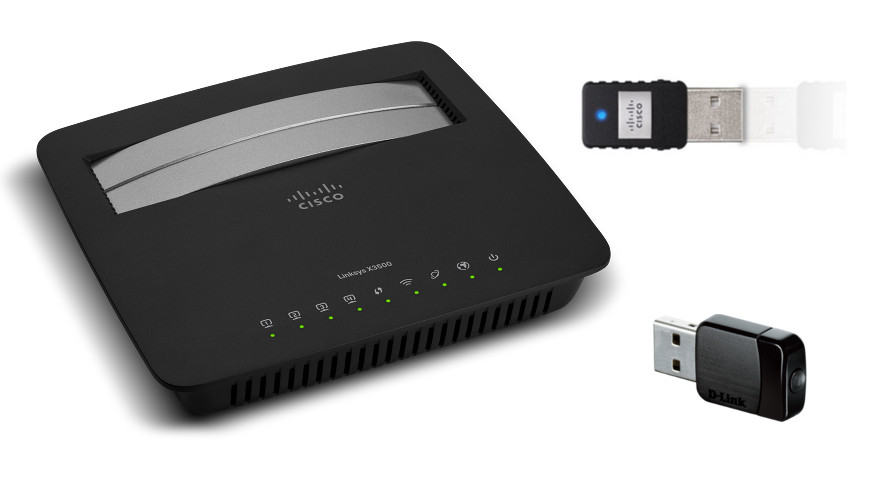
\includegraphics[width=0.5\textwidth]{../Images/c2/hardware_comm.jpg}
	\caption{WiFi PA and USB adapters}
	\label{fig:hardwareComm}
\end{wrapfigure}

En esta secci\'on se describe brevemente la arquitectura de comunicaci\'on \ref{chap:c6_network}. La red tiene un doble uso, en primer lugar la interconexi\'on de las diferentes partes del sistema y en segundo lugar al generarse una capa de abstracci\'on con las comunicaciones los sistemas pueden ser probados en cualquier sistema operativo y a trav\'es de cualquier m\'odulo de comunicaci\'on (Adaptadores WiFi, m\'odulos GSM, etc).

%----------------------------------------------------------------
\subsection{Software, protocol and messages}

\begin{wrapfigure}{r}{0.5\textwidth}
	\begin{center}
		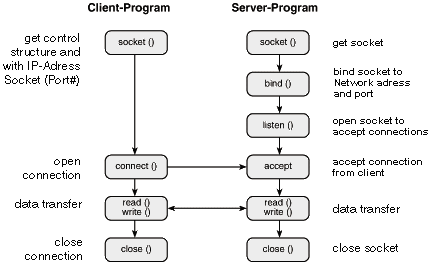
\includegraphics[width=0.5\textwidth, natwidth=448, natheight=263]{../Images/c2/socketstcpip.png}
	\end{center}
	\caption{Sockets y TCP-IP}
	\label{fig:socketstcpip}
\end{wrapfigure}

Para la comunicaci\'on entre procesos se usa una implementaci\'on de sockets TCP/IP \cite{TCPIP} incluida en la librer\'ia \cite{BOViL}.\\
Cada paso del algoritmo de visi\'on se generan centroides correspondientes a los objetos. Estos se almacenan en un vector que se manda a trave\'es del socket byte a byte con el siguiente formato \{App;quadID;color;centroids\}. Por ejemplo $\{14;01;5;123-231,142-22,...,600-232\}$

